\chapter{Informationsbeschaffung}
\label{Informationsbeschaffung}
 In einer ersten Phase wurde ein Zeitraum zur Informationsbeschaffung festgelegt. Dieser Abschnitt ist einerseits für die Themeneinarbeitung und anderseits für die Absteckung der Aufgabe und der Ziele erforderlich.

Nachfolgend werden die wichtigsten Erkenntnisse der Informationsbeschaffung erläutert, die maßgebend für die Konzeption in Kapitel \ref{chap:Konzeption} und die Realisierung in Kapitel \ref{chap:Realisierung} sind. Dabei werden zu einzelnen Komponenten und Verfahren Stellung genommen und eruiert, ob diese sich für das Projekt eignen. Des Weiteren werden relevante Software erläutert, welche für die Realisierung nötig sind. Ein weiterer Abschnitt behandelt bereits bestehende State-of-the-Art-Lösung.


\section{Entfernungsmessung}
\label{sec:Entfernungsmessung}
In diesem Unterkapitel werden die bestehenden Entfernungsmesser Hokuyo URG-LX04 und der Velodyne VLP-16 beschrieben. Dabei werden wichtige Spezifikationen erläutert. Für die Aufgabenstellung wurde von Herr Jensen der Velodyne VLP-16 ausgewählt, daher wird nur kurz auf den Hokuyo URG-04LX eingegangen. Es soll erläutern, weshalb der Velodyne VLP-16 für das Projekt besser geeignet ist.

\subsection{Hokuyo URG-04LX}
\label{subsec:Hokuyo}
Der Hokuyo URG-04LX ist ein zweidimensionaler Entfernungsmesser, der mittels \ac{LIDAR} Verfahren misst. Bei diesem Verfahren wird mit reflektierten Laserimpulsen die Entfernung eruiert. Nachfolgende Angaben entstammen aus den Datenblättern. \cite{hokuyo} 

Wie in Abbildung \ref{fig:URG-04LX} ersichtlich, bietet der Laserscanner eine Abdeckung von 240 Grad in eine definierte Evene. Dabei benötigt dieser 100 ms pro Scan. Die zu erwartende Auflösung liegt dabei bei 1 mm. Die gemessenen Daten werden über eine USB-Schnittstelle übermittelt, direkt nachdem der Scan vollführt wurde.

\begin{figure}[H]
	\centering
	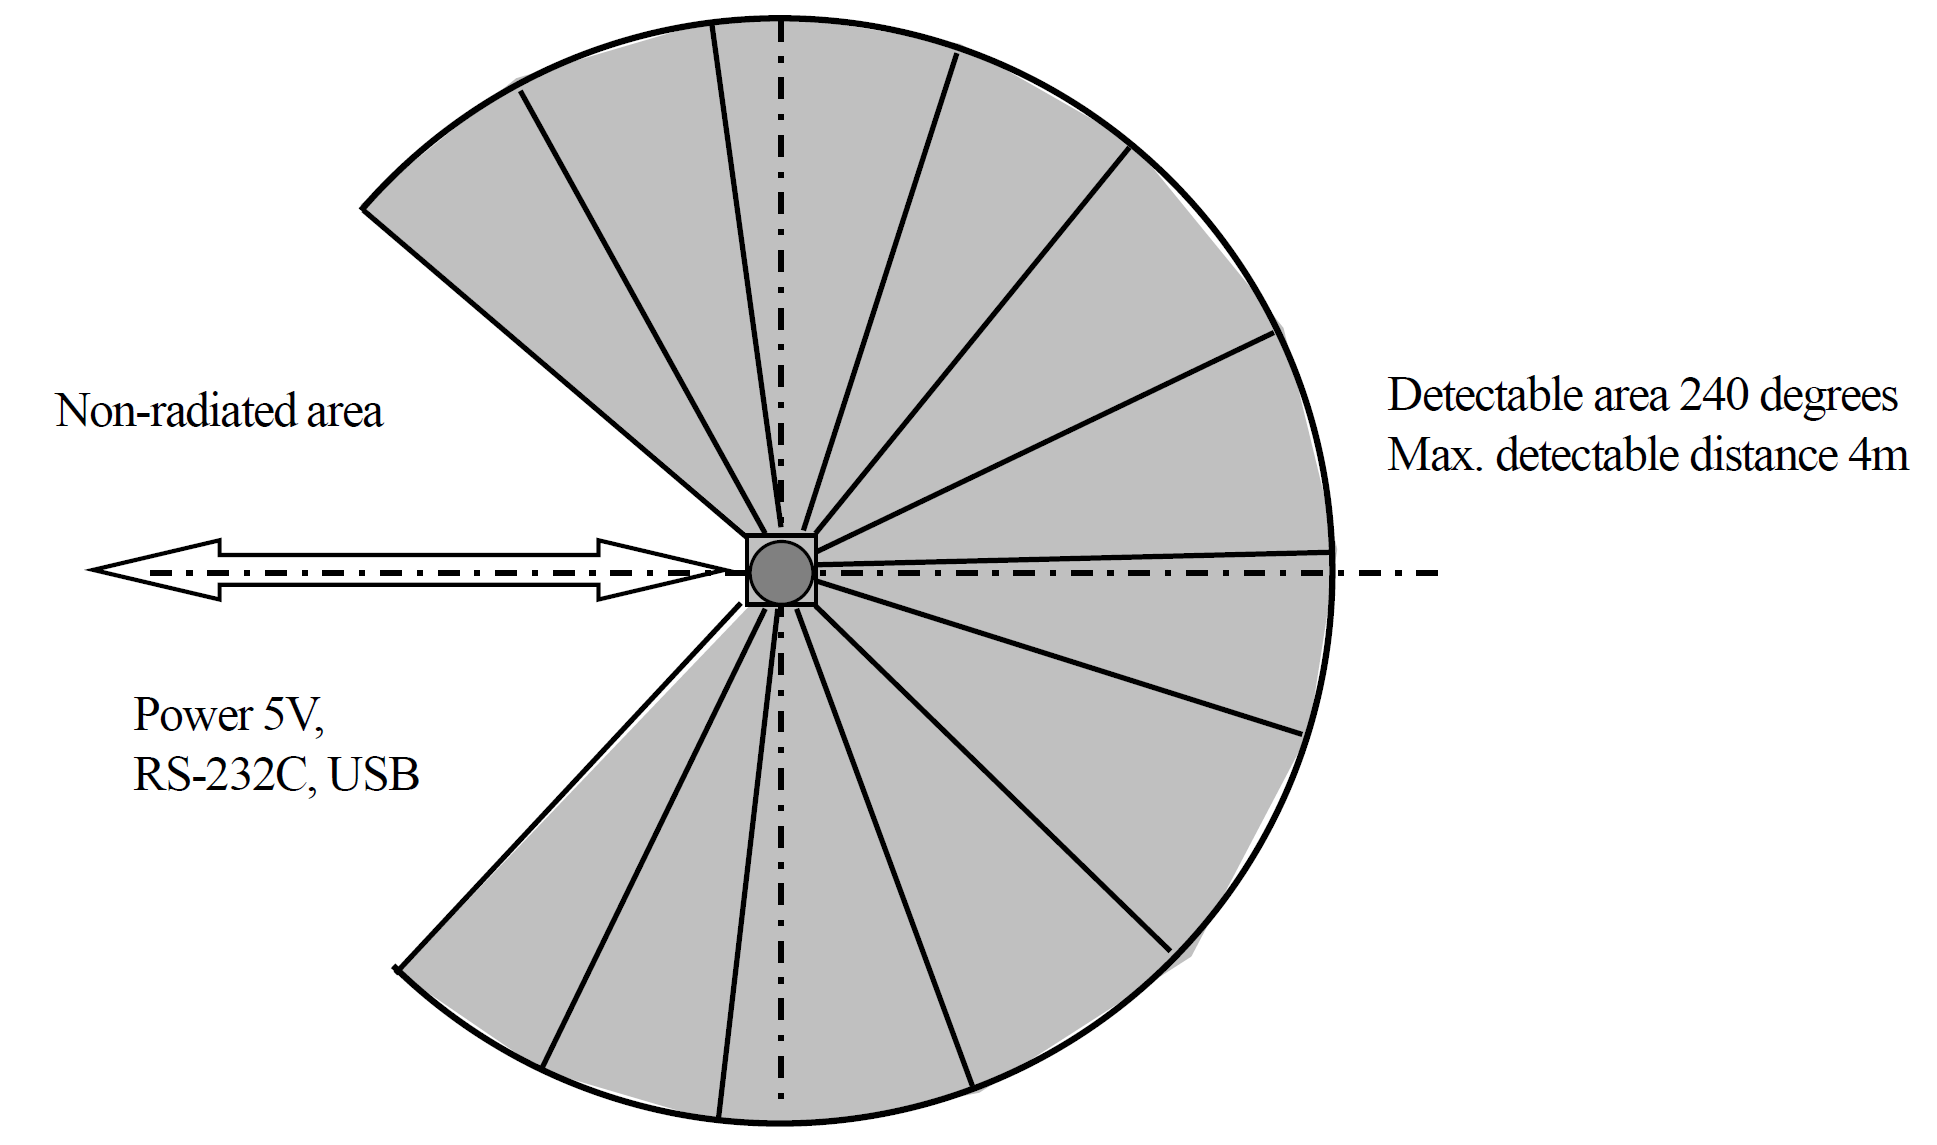
\includegraphics[width=0.5\textwidth]
	{resources/detectableAngle.PNG}
	\caption[messbarer Bereich]{messbarer Bereich} \protect\cite{hokuyo}
	\label{fig:URG-04LX}
\end{figure}

\todo{ref}
Ein bedeutendste Nachteil des URG-04LX für die Aufgabenstellung ist das messbare Distanzspektrum. Die maximale Messdistanz von 4 m genügt nur für sehr nahe räumliche Messungen. Der Einsatzbereich beschränkt sich hier lediglich für Gebäude interne Messungen. Da mit dem dem zu erarbeitenden Modul Umgebungskarten erstellt werden sollen, eignet sich dieser Laser nicht.

\subsection{Velodyne VLP-16 Puck}
\label{subsec:Velodyne}
Beim Velodyne VLP-16 Puck handelt es sich um einen Echtzeit 3D-Laser-Scanner, der auf dem \ac{LIDAR}-Verfahren basiert. Nachfolgende Angaben entstammen den Datenblattangaben, wenn nicht anders referenziert. \protect\cite{velodyne}

Der VLP-16 bietet insgesamt 16 Laser-/Detektorpaare, die in \ref{fig:angleVLP} ersichtlich sind. Mit diesen wird in horizontaler Lage eine Abdeckung von 360 Grad erreicht. Dies wird dadurch ermöglicht, dass der Laserscanner sich intern mit 5 - 20 Rotationen pro Sekunde um die eigene Achse dreht. Die Rotationsgeschwindigkeit ist dabei einstellbar. Dabei kann mit einer horizontalen Auflösung von 0.1 \degrees – 0.4\degres gerechnet werden.
Die vertikale Abdeckung hingegen ist auf 30 \degres begrenzt. Da die 16 Laser mit je 2 \degres Unterschied ausgerichtet sind ergibt sich daraus 30 \degres mit einer vertikalen Auflösung von 2 \degres. Ein wichtiger Punkt ist somit, dass zwischen den Laserstrahlen keine Messpunkte ermittelt werden können, um diese zu ermöglichen müsste er seine Position verändern können, damit könnte auch die vertikale Abdeckung erweitert werden. 

\begin{figure}[H]
	\centering
	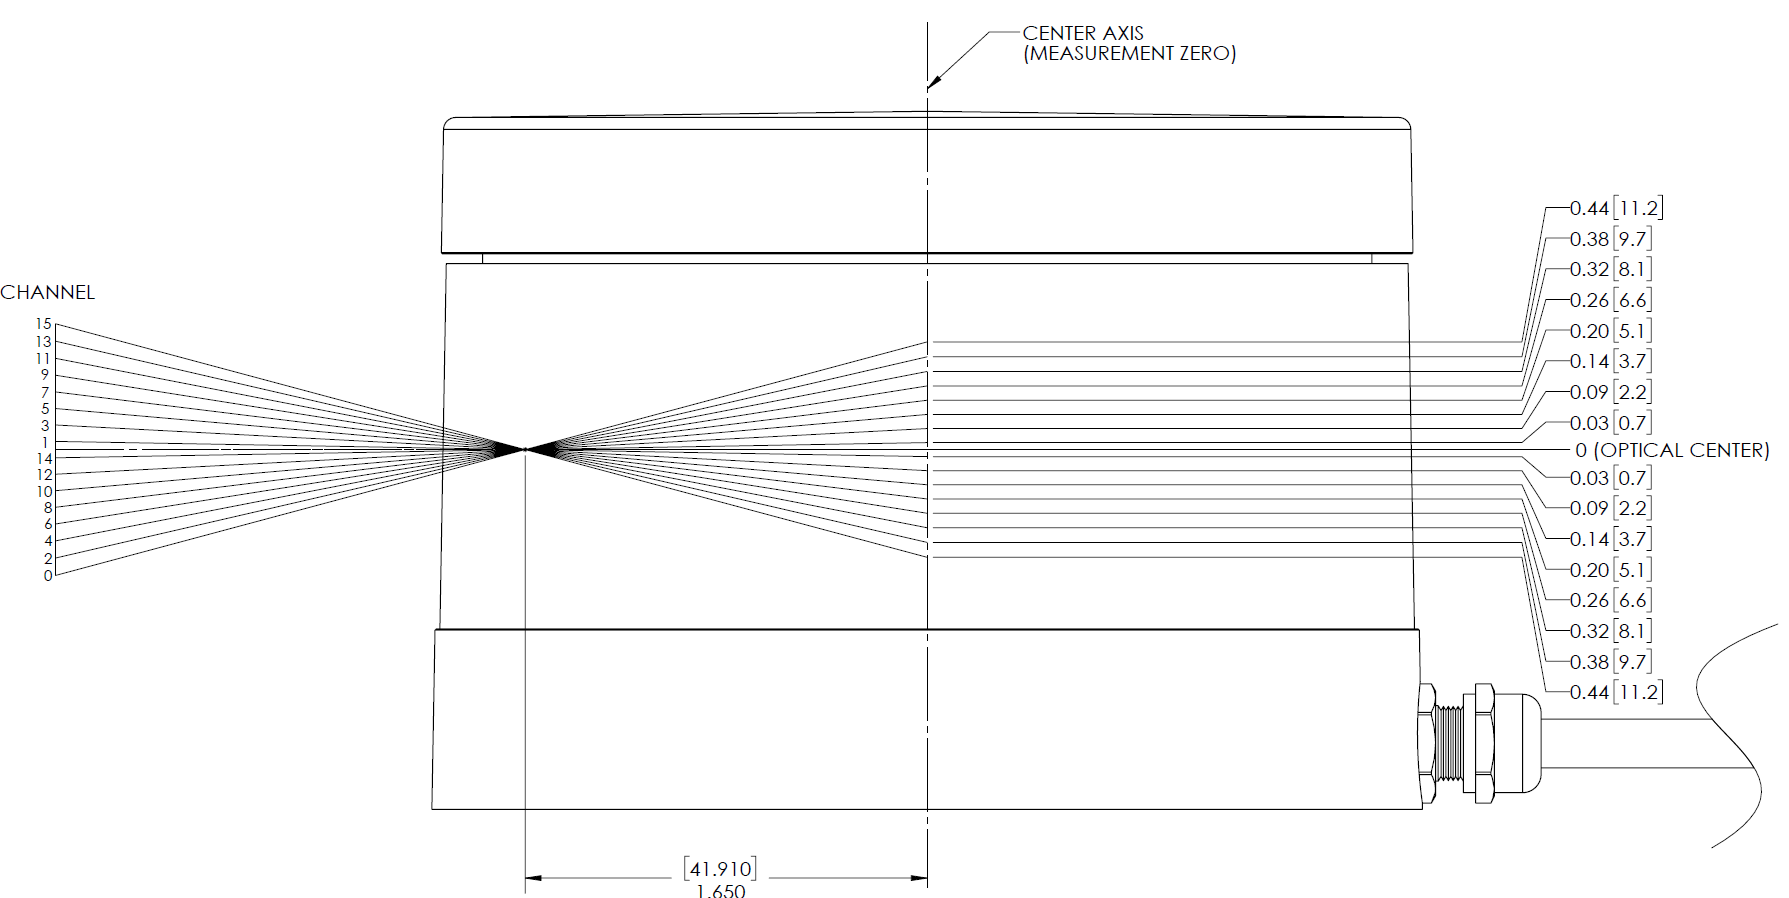
\includegraphics[width=0.6\textwidth]
	{resources/velodyne_channels.PNG}
	\caption[Laserstrahlen des Velodyne  VLP-16]{Laserstrahlen des Velodyne  VLP-16} \protect\cite{velodyne}
	\label{fig:angleVLP}
\end{figure}

Ein besondere Eigenschaft dieses Laserscanners ist die vergleichbar grosse Messdistanz, die Distanzen  zwischen 1m bis 100 m ermöglicht. Dabei ist die die typische Toleranz +/- 3 cm. Zusätzlich wird der Reflektionsgrad in 256-bit Auflösung gemessen.    

Der VLP-16 benötigt eine separate Interface Box, da die Speisung und Datenübertragung des 8-adriges Anschlusskabel getrennt werden muss. In \ref{fig:CablePin} ist dieses Kabel mit Pinbelegung dargestellt. Dabei werden die Adern 1-4 für die Ethernet Datenübertragung benötigt. Die Adern 5 und 6 sind nur bei zugeschaltetem \ac{GPS} nötig, ansonsten sind diese unbenutzt. Die stabilisierte 12 Volt Spannung wird über die Adern 7 und 8 zugeführt.

\begin{figure}[H]
	\centering
	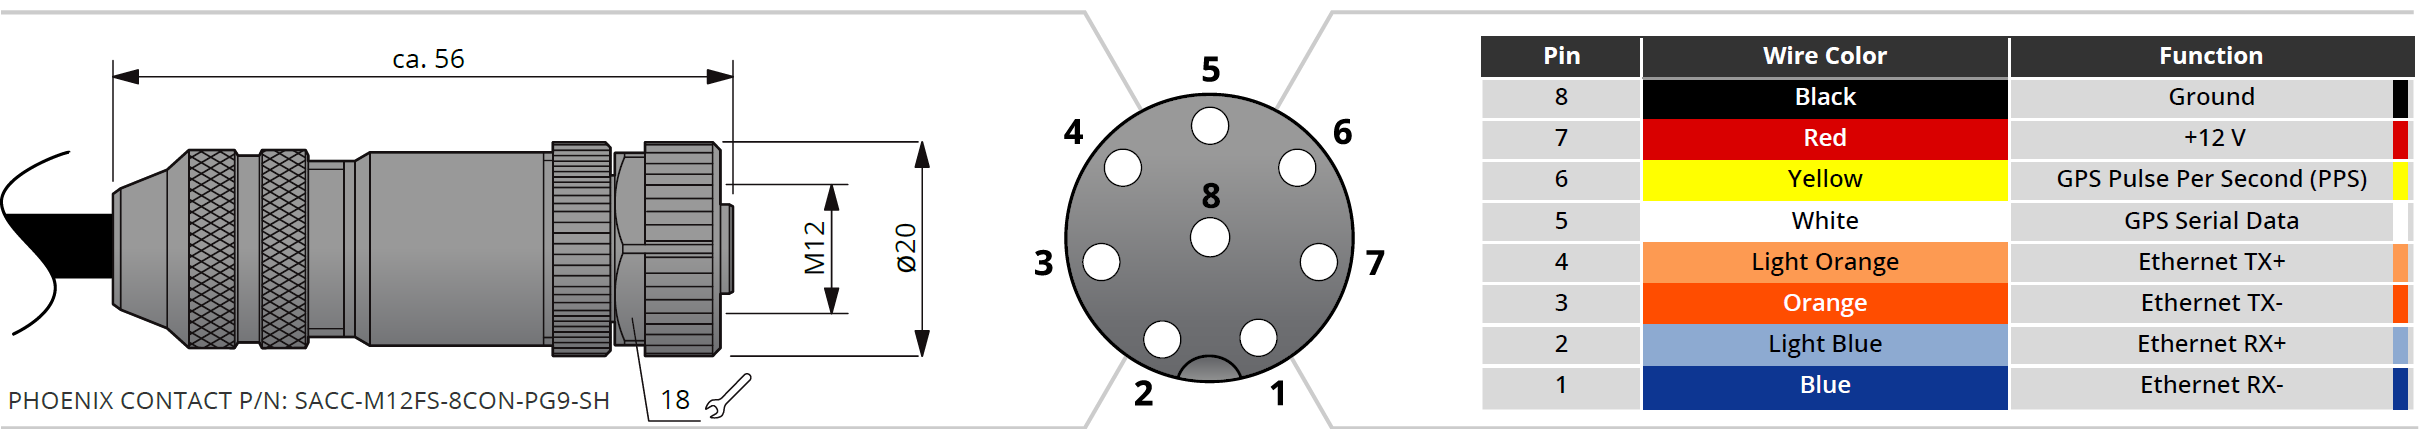
\includegraphics[width=1\textwidth]{resources/Cablepins.PNG}
	\caption[Anschluss und Kabelbelegung]{Anschluss und Kabelbelegung}\protect\cite{velodyne}
	\label{fig:CablePin}
\end{figure} 

Die Interface Box ist in \ref{fig:InterfaceBox} ersichtlich.  Diese besitzt folgende Anschlüsse; 12 Volt Speisung, sowie ein Ethernet RJ45 Anschluss und eine \ac{GPS} Schnittstelle. Die typische Leistungsaufnahme des Sensors ist hierbei 8 Watt.

\begin{figure}[H]
	\centering
	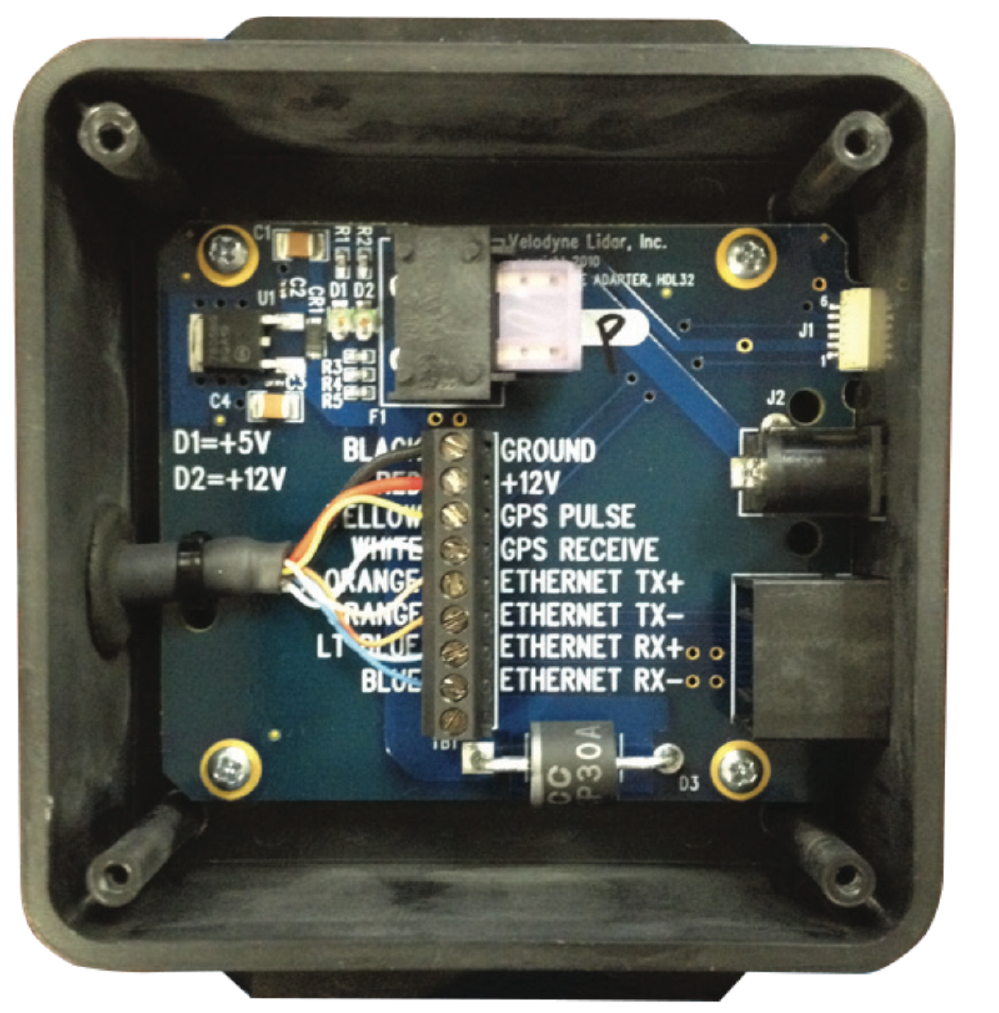
\includegraphics[width=0.4\textwidth]
	{resources/InterfaceBox.PNG}
	\caption[Ansicht auf die Interfacebox]{Ansicht auf die Interface Box} \protect\cite{velodyne}
	\label{fig:InterfaceBox}
\end{figure}

Über die 100 Mbps Ethernetverbindung werden die Daten- und Positionspakete vom Velodyne an den Computer übermittelt. Dabei werden für die zwei verschiedene \ac{UDP} Pakets die Ports 2368 und 8308 gebraucht. Nachfolgend wird in \ref{fig:datenpakets} der Aufbau eines Datenpakets dargestellt. Jedes Paket besitzt einen 42-Byte Header und einen Datenblock, der aus Laserrückgabewert, kalibrierten Reflektionsgrad, Azimutwert und Zeitstempel besteht.

\begin{figure}[H]
	\centering
	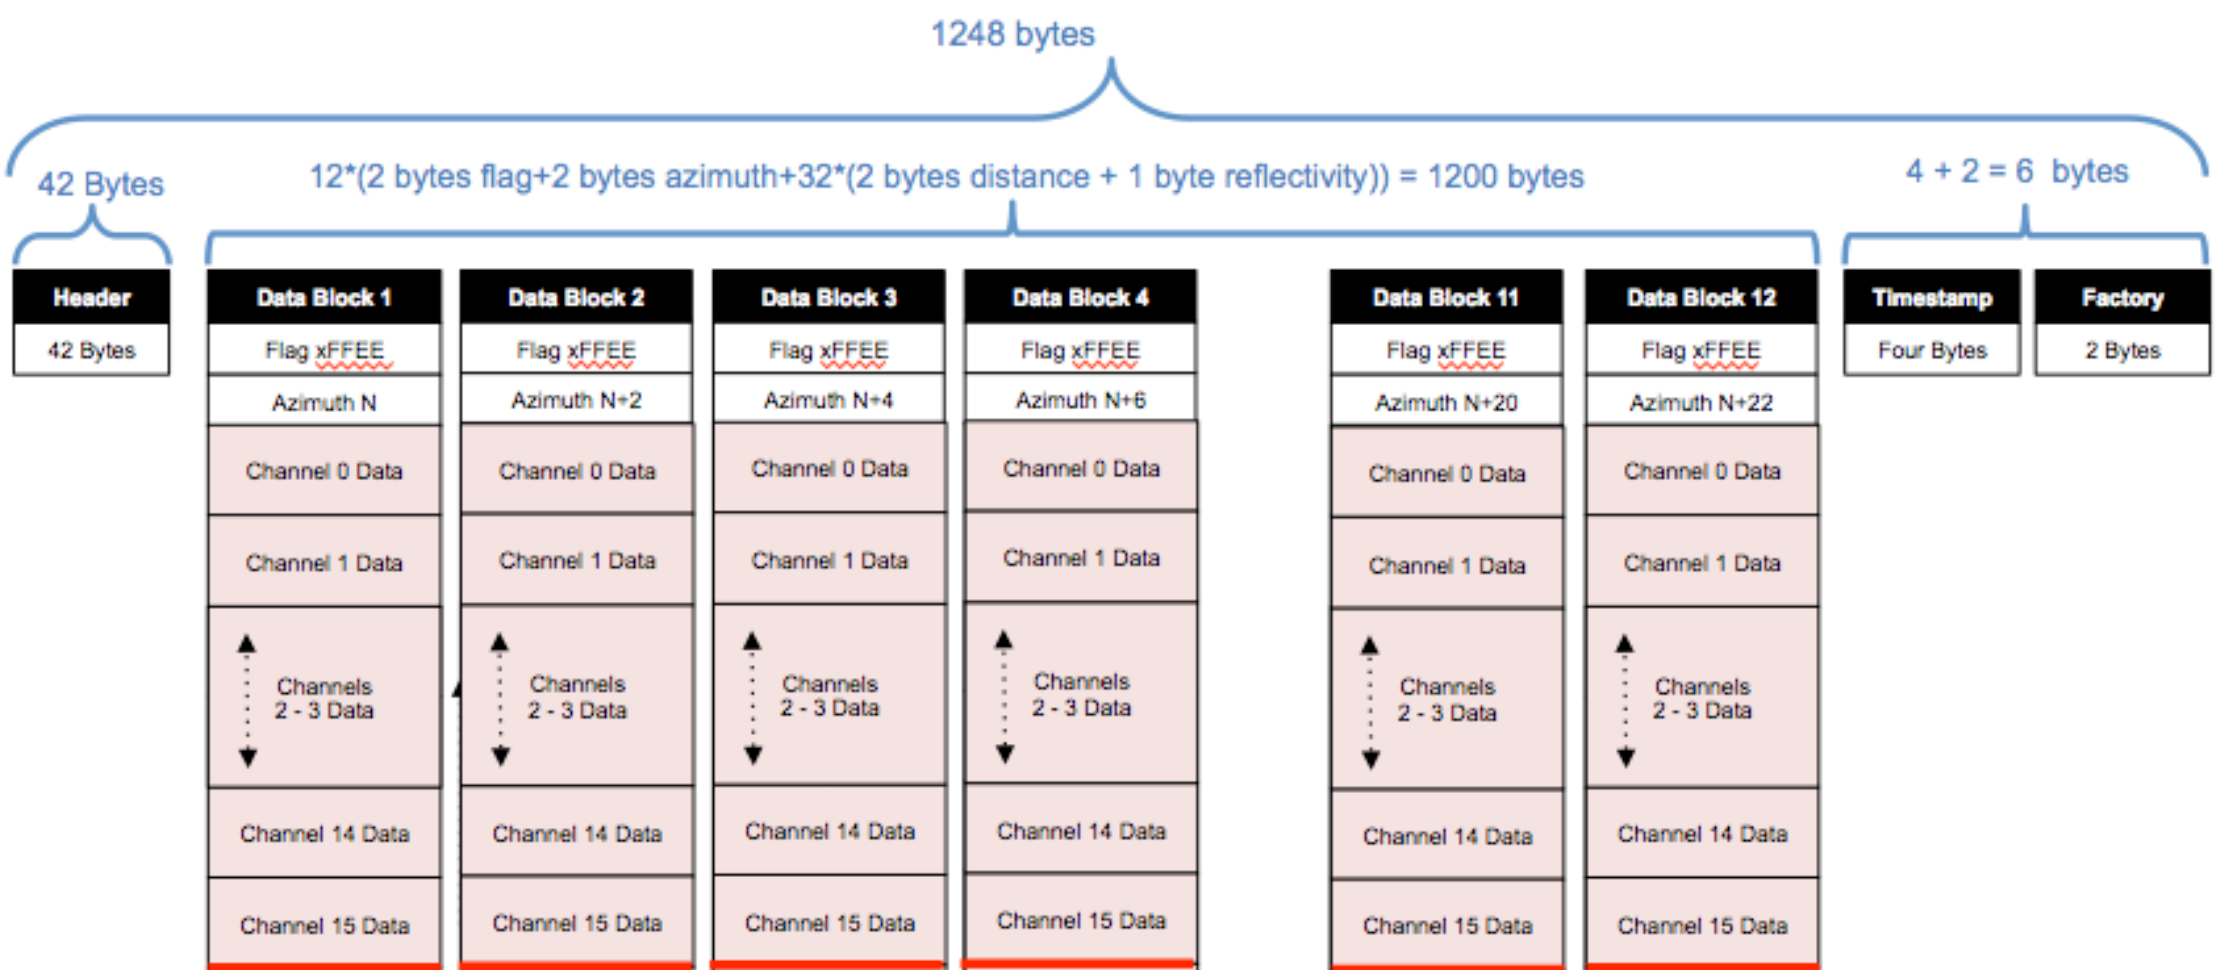
\includegraphics[width=1.0\textwidth]
	{resources/datapakets.PNG}
	\caption[Aufbau Datenpaket]{Aufbau Datenpaket} \protect\cite{velodyne}
	\label{fig:datapakets}
\end{figure}


\section{Vorzeigeprojekte}
 	\label{sec:Vorzeigeprojekte}
 Dieses Kapitel dient als Vorstudie über den Einsatz des Velodyne VLP-16 durch bereits bestehende Projekte. Dabei werden zwei verschiedene Konfigurationen betrachtet und dazu entsprechend Vor- und Nachteile erläutert. Es handelt sich hierbei um zwei Teams, welche an der \ac{EnRicH} 2017 teilgenommen haben und als State-of-the-Art betrachtet werden.
 
 
 \subsection{IMM MSAS Team MSS Warschau}
 	\label{subsec:IMM}
 Das Institute of Mathematical Machines (IMM) in Warschau hat den Velodyne VLP-16 an einer endlos drehenden Konstruktion befestigt. Dabei ist der Sensor nicht in der üblichen Lage (Ausrichtung XY-Ebene), sondern um 90 \degrees abgedreht (Ausrichtung YZ Ebene). In Abbildung \ref{fig:imm} ist die entsprechende Konfiguration abgebildet. 
Für die nachfolgenden Betrachtungen wird nur der 0 \degrees ausgerichtete Laserkanal 1, siehe Abbildung \ref{fig:angleVLP}  dargestellt. Der Laserstrahl dreht mit der Winkelgeschwindigkeit  um den Radius Rv. Dabei ermittelt er Azimut und Reflektionsgrad. Wird die Konstruktion nun konstant im Uhrzeigersinn gedreht wird die Ausrichtung des Laserkanals 1 kontinuierlich verändert. Dabei entspricht der Laserkanal einem Drehzeiger mti der Distanz

Es entsteht folgende homogenene Transformationsmatrix 

\todo{Transformationsmatrix}



 
 Durch die Lage des Velodyne kann folgende homogene Transformation ermittelt werden.
 
  Der Vorteil dieser Konstruktion ist, dass durch die endlose Rotation um die Z-Achse Messpunkte rund um den Roboter ermittelt werden kann, da sich die zu  16
   
  
   \begin{figure}[H]
  	\centering
  	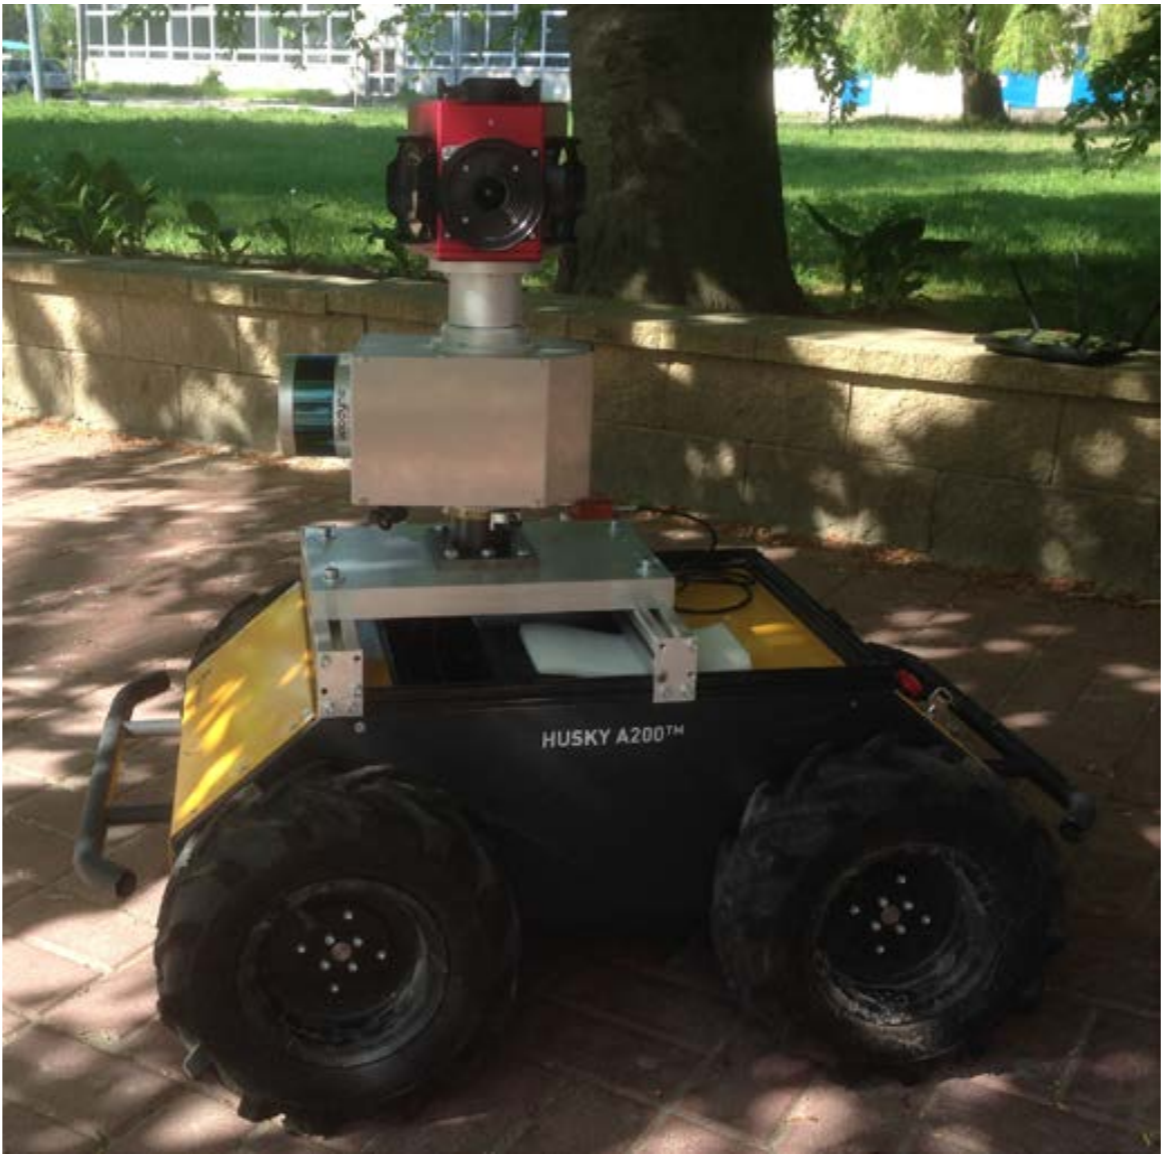
\includegraphics[width=0.6\textwidth]
  	{resources/IMM.PNG}
  	\caption[Roboter des Team IMM EnRicH]{Roboter des Team IMM an der EnRicH} \protect\cite{velodynee}
  	\label{fig:imm}
  \end{figure}
  
  Diese Konfiguration besitzt jedoch den Nachteil, dass viele Messpunkte in Richtung Fahrzeug und in Richtung Z-Achse ermittelt werden. Es können somit auch hohe Objekte mit kurzer Entfernung zum Roboter detailliert vermessen werden. Im freien Feld bietet diese Konfiguration jedoch den Nachteil, dass viele Messpunkte ins Leere messen, vor allem in die Z-Achse (himmelwärts). Des Weiteren werden viele Messpunkte in Richtung -Z (Roboter) vermessen, die für das Mapping keine Resultate liefern, da sich in dieser Richtung der Roboter befindet 
 

 	
  \subsection{Hector Tracker Team Hector Darmstadt}
 \label{subsec:hector}
Das Team Hector der Universität Darmstadt besitzt auf dem Hector Tracker eine weitere Konfigurationsmöglichkeit. Auch dieses Team arbeitet mit einem endlos drehenden Konstruktion. Der Velodyne VLP-16 befindet sich 45\degres abgeneigt zur XZ-Ebene. Dabei ist die Lage des Sensors zentral auf der Drehachse Z.

Der Vorteil dieser Konstruktion ist das durch die 45 Grad Stellung des VLP-16 und der zusätzlichen Rotation um die Z-Achse ein breitere Abdeckung entsteht. Während einer Umdrehung kann 

Im Vergleich zum Projekt der IMM entstehen bei dieser Konfiguration weniger Messpunkte in Richtung des Roboters und in in die Richtung Z-Achse (himmelwärts).



\begin{figure}[H]
	\centering
	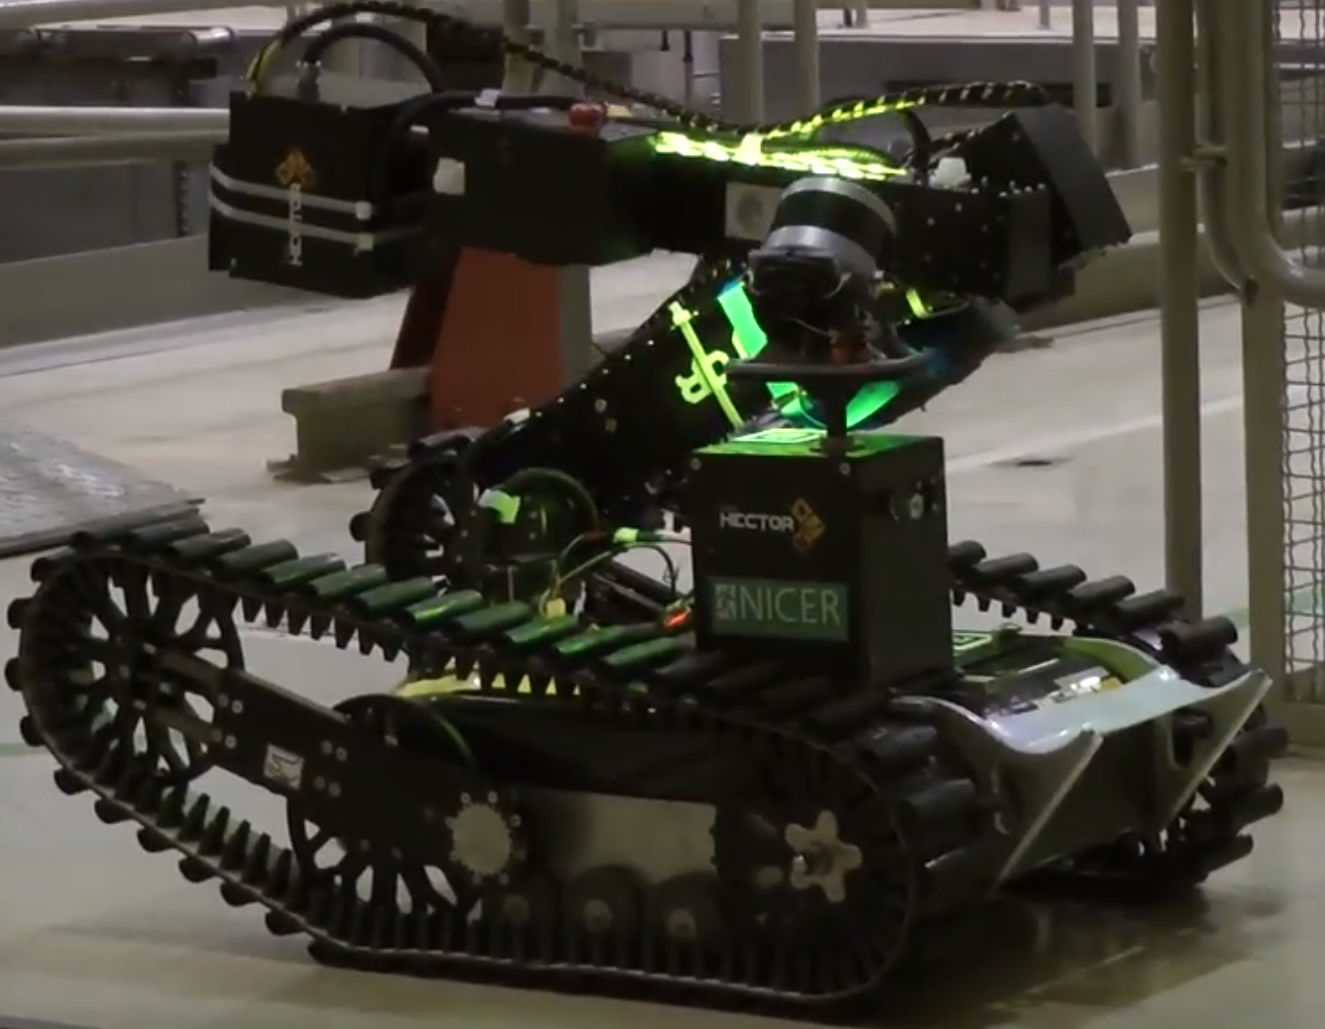
\includegraphics[width=0.8\textwidth]
	{resources/hector.PNG}
	\caption[Roboter des Team Hector EnRicH]{Roboter des Team Hector an der EnRicH} \protect\cite{velodyne}
	\label{fig:hector}
\end{figure}


%% http://enrich.european-robotics.eu/documents/ENRICH_TeamInformation-IMM.pdf
 	
  \subsection{Schlussfolgerung}
  An der EnRicH nahmen insgesamt 11 Teams teil. Dabei nutzen mehrere Teams den Velodyne VLP-16 mit unterschiedlichen Konfigurationen. Die zwei betrachteten Konfigurationen nutzen die Möglichkeit einer endlos drehenden mechanischen Konstruktion. im Abschnitt \ref{sec:Antriebsmoeglichkeiten} werden mögliche Antriebsmöglichkeiten evaluiert.
  
 

\section{Software}
\label{sec:Software}
In diesem Kapitel wird die notwendige Software beschrieben. Es erläutert einerseits das \ac{ROS} und dessen Funktion im Projekt. Daneben werden kurz weitere Softwareapplikationen und -packages erwähnt, welche während der Erarbeitung nützlich sind.

\subsection{ROS Robot Operating System}
\label{subsec:ROS}
Die gesamte Kommunikation mit Sensoren und Aktoren findet auf dem Packbot mit einem spezifisch implementierten \ac{ROS} statt. Daher ist es naheliegend, um die Integrität des zu erarbeitenden 3D-Laser-Moduls zu gewährleisten, dieses Software-Framework zu nutzen.  

\subsection{ROS Kinetic Kame vs. Indigo}
\label{subsec:OS_versus} 
Grundsätzlich wird \ac{ROS}, wegen seiner Nähe zu Linux Distributionen, auf einem Ubuntu Betriebssystem aufgesetzt und ist ein grösstenteils Kommando-basiertes Software-Framework. Diese in 2007 entwickelte Open Source Software erhielt in den letzten Jahren ständig neue und überarbeitete Versionen. In der nachfolgenden Abbildung sind die aktuellen Distributionen ersichtlich.

\begin{figure}[H]
	\centering
	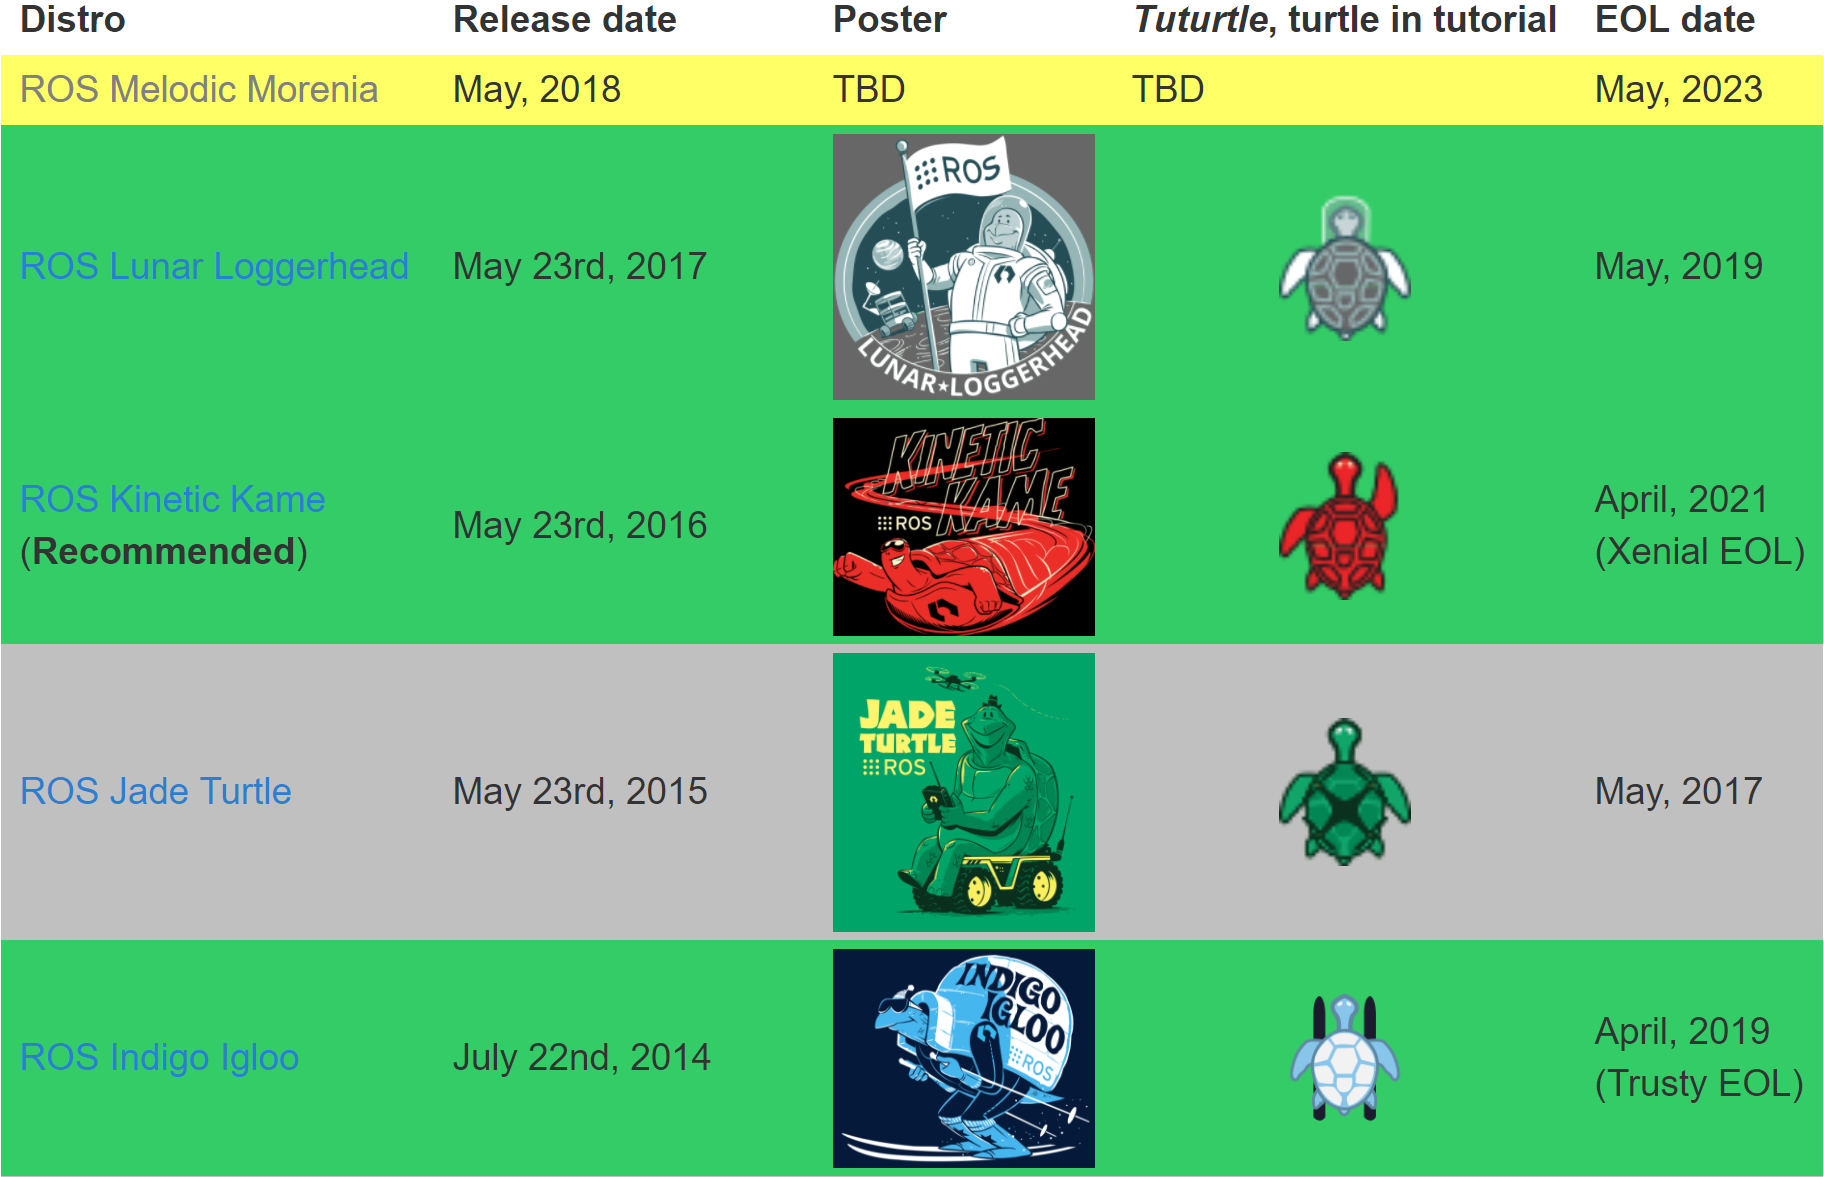
\includegraphics[width=0.6\textwidth]{resources/rosdistos.PNG}
	\caption[aktuelle Distributionen von ROS]{aktuelle Disttributionen von ROS {\cite{ROSprojects}}}
	\label{fig:rosdistros}
\end{figure} 

Die Empfehlung von ROS und diversen Literaturen liegt hierbei bei der neusten Distribution ROS "Kinetic Kame". Es handelt sich hierbei um eine Langzeitversion von ROS, welche bis 2021 Unterstützung bietet. Im Zug der ersten Versuchen mit ROS wurde auf einem Laptop mit AMD64-Architektur gearbeitet. Auf diesem wurde ROS Kinetic Kame vollumfänglich ermöglicht. Für das 3D-Lasermodul wird jedoch ein einbaubaren Einplatinencomputer benötigt, welche im \ref{sec:Datenverarbeitung} genauer betrachtet werden. 

Während der Einarbeitung mit Kinetik Kame konnten einige Nachteile der Distribution festgestellt werden. Kinetik Kame unterstützt offiziell die erforderliche Velodyne Packages für den VLP-16 noch nicht. Diese können jedoch über einen unoffiziellen Github Account von DataSpeed Inc. bezogen werden. Dabei wurde jedoch festgestellt, dass zum Teil inoffizielle Packages nur für amd64-Architekturen zur Verfügung stehen. Dies ist ein wesentlicher Nachteil, da die meisten Einplatinencomputer mit ARM-Architekturen arbeiten.
\todo{Erkentnisse 01.11.2017}

Der Vorgänger ROS Indigo unterstützt offiziell die Velodyne Packages. Dabei muss jeodch berücksichtigt werden, dass Indigo nur auf Ubuntu 14.04 Trusty Truh läuft. ROS Indigo wird nur noch bis April 2019 unterstützt, bietet jedoch im Vergleich zu allen Distributionen die meisten offiziellen Packages, da es bereits 2014 veröffentlicht wurde. 
 
\subsection{Point Cloud Library}
\label{subsec:PointCloudLibrary}
Die Point Cloud Library (PCL) ist eine freie Programmbibliothek mit zahlreichen Algorithmen zur Verarbeitung n-dimensionaler Punktwolken und dreidimensionaler Geometrien.

Ein wesentlicher Vorteil dieser Programmbibliothek ist die Integration in ROS.
\subsection{Wireshark}
\label{subcec_Wirehark}
\todo{evlt}
\subsection{Onshape}
\label{subsec:OnShape}
\todo{evlt}

\section{Datenverarbeitung}
\label{sec:Datenverarbeitung}
Um die Datenmenge zu verarbeiten und die Ansteuerung der Komponenten zu realisieren eignen sich Einplatinencomputer. In diesem Zusammenhang werden nachfolgend diverse Einplatinencomputer betrachtet. Kriterien bei der Auswahl eines geeigneten Boards sind Prozessorleistung, Preis, Ethernet-Schnittstelle, Speichermöglichkeit, GPIO Verfügbarkeit und die verbaubare Dimension. 

\subsection{Raspberry Pi 2 \& 3}
\label{subsec:Raspberry}
Das Raspberry Pi ist eines der bekanntesten Einplatinencomputer und bietet daher eine grosse Community. Da bereits ein Raspberry Pi 2 zur Verfügung gestanden ist, konnten die ersten Erfahrungen mit einem Raspberry Pi gemacht werden. Das Raspberry bietet zusammen mit ROS Kinetic Kame und Ubuntu Mate LTS 16.04 eine mögliche Lösung für die Datenverarbeitung. Das Raspberry Pi 2 bzw. 3 basiert auf einem Broadcom \ac{SOC} und ist mit einem ARM Cortex A7 bzw. A53 Prozessor mit vier Kernen ausgestattet. Die Taktfrequenz liegt bei diesen lediglich bei 1.2 GHz. Beide Modelle besitzen 1 GB RAM. Das Betriebssystem wir auf einer \ac{SD}-Card gebootet.
\todo{Ergäenzung erkenntnisse}  

\subsection{Banana Pi M3}
\label{subsec:BananaPi}
Der Banana Pi M3 bietet zur Zeit (Stand Oktober 2017) die höchste Performance bei Einplatinencomputern mit ARM-Architektur durch den Allwinner A83T Achtkern-Prozessor, der mit 1.8 GHz taktet. Neben USB-Anschlüssen bietet es eine SATA-USB-Schnittstelle, die den internen 8 GB \ac{eMMC}-Speicher um bis zu 2 TB erweitern lässt. Es bietet auch direkt integrierte WLAN-Schnittstellen, sowie eine RJ45 Gigabit Netzwerkschnittstelle. Zum Betreiben des Banana PI M3 benötigen man ein 5V DC-Netzteil. Der Preis eines BananaPi M3 liegt momentan bei ca 90. Franken. In Zusammenhang mit Ubuntu 

 
\subsection{Odroid C2 \& XU4} 
\label{subsec:Odroid}
In diversen Literaturen (siehe \cite{ROSprojects} Kapitel 4) werden neben dem Raspberry Pi, Odroid Boards als empfohlene Einplatinencomputer aufgelistet. Dabei stehen die aktuelle Modelle Odroid-C2 oder Odroid-XU4 zur Verfügung. Sie bieten eine höhere Prozessorleistung, 1.5 GHz bzw. 2 GHz mit je 2 Gigabyte \ac{RAM}. Betribssysteme können via \ac{SD} oder \ac{eMMC} gebootet werden. Beide Boards sind jedoch noch nicht lange auf dem Markt und bieten in vielen Anwendungen nur Beta-Versionen. Vor allem die Unterstützung von Ubuntu LTS 16.04 ist nicht restlos geklärt. Der Preis dieser Boards ist um die 80 - 90 Franken.

\subsection{Lattepanda} 
\label{subsec:Lattepanda}
Der Lattepanda Einplatinencomputer unterscheidet sich wesentlich von den bisherig betrachteten Boards. Der Prozessor arbeitet nicht mit ARM-Architektur, sondern mit Amd64-Architektur. Somit können Ubuntu und ROS Distributionen voll umfänglich genutzt werden. Der Intel Atom ist ein vier kerniger Prozessor und taktet mit 1.84 GHz. Zusätzlich bietet es einen separaten 500 MHz \ac{GPU}  und 4 GB \ac{RAM}. Es bietet neben USB, RJ45 auch einen ATMmega 32u4 Coprozessor, mit welchem 20 GPIO headers angestuert werden können. der Preis eines Lattepanda kostet je nach Ausführung zwischen 130 -180 Fr.

\subsection{Up Board Squared}
\label{subsec:UpBoard}
Das Up Board Square arbeitet wie das Lattepanda mit einer Amd64-Architektur 


\section{Antriebsmöglichkeiten}
\label{sec:Antriebsmoeglichkeiten}
Um das Produkt um eine Achse drehen zu lassen, müssen Motoren eingesetzt werden. Nachfolgend sind zwei verschiedene Motorenarten geschildert, um die Einsatzmöglichkeit zu klären. Wichtige Kriterien für die Aufgabenstellung sind einerseits die Ansteuerung und die Dimension. Anderseits muss die Möglichkeit bestehen die Winkeländerung zu eruieren. 

\subsection{Schrittmotor}
\label{subsec:Schrittmotor}
Der Schrittmotor ist eine Antriebsmöglichkeit, welche für das Projekt in Frage kommt. Es gibt sehr kostengünstige und kompakt dimensionierte Motoren dieser Art. Ein interessanter Aspekt ist das gezielt Steuern des Motors. Durch einen Stromimpuls bewegt sich ein Schrittmotor nur einen festgelegten Winkelschritt weiter. Er kann bereits ohne zusätzliche Sensorik definierte Schritte anfahren, aus denen die Winkeländerung eruiert werden kann. Schrittmotoren besitzen die Eigenschaft, dass in der Ruhelage ein Haltemoment entsteht. Diese Eigenschaft wird jedoch für die Aufgabenstellung nicht zwingend benötigt. 

Nachteilig für die Aufgabenstellung am Schrittmotor ist der höhere Stromverbrauch, vor allem während dem Haltemoment. Da nur ein Schritt vollführt werden kann, wenn das entsprechende Drehmoment nicht überschritten wird, müsste dieses sorgfältig berechnet werden. Ein bedeutender Nachteil im Zusammenhang mit der Aufgabenstellung ist, dass durch Schrittverluste die Winkeländerung nicht mehr quantitativ ermittelt werden kann.
Ein weiterer Nachteil ist das verhältnismäßig hohe Gewicht. Dies ist kein Kriterium für die Aufgabenstellung, sollte jedoch bei der Realisierung beachtet werden.

Um mit einem Mikrocontroller einen Schrittmotor anzusteuern, empfiehlt sich ein Schrittmotorentreiber. Mit solchen Treibern lässt sich der Motor mittels 2 Steuerpins rotieren. Um die Drehgeschwindigkeit zu senken, bieten diese Treiber die Möglichkeit, die Schritte in 2, 4, 8 und 16 Teilschritte zu senken,um dadurch eine feinere Bewegung zu ermöglichen. 

\subsection{Gleichstrommotor}
Als Alternative zum Schrittmotor bietet sich ein üblicher Gleichstrommotor. Diese Motoren sind für viele Einsatzbereiche geeignet und es gibt sie in verschiedenen Grössen und Umdrehungszahlen. Im Gegensatz zu Schrittmotoren laufen Gleichstrommotoren kontinuierlich, aufgrund eines Stroms, der durch die Wicklungen fliesst. Nachteilig ist somit, dass weder die genaue Anzahl Umdrehungen noch die momentane Phasenlage bekannt ist. Es gibt jedoch eine Vielzahl an Möglichkeiten diese zu eruieren. Einerseits gibt es die Möglichkeit mittels Hall-Sensoren oder mittels Quadraturencodern, die aktuelle Drehrichtung und die Drehzahl zu ermitteln. Um dies zu ermöglichen, braucht es zusätzlich einen Vierquadrantensteller (H-Brücke), sowie eine Sensorlogik, damit der Sensor mittels \ac{PWM} angesteuert werden kann. Im Preissegment bis 40 Fr. gibt es leistungsfähige Gleichstrommotoren für den Anwendungsbereich.


\section{Speisung und Verkabelung}
\label{sec:Speisung und Verkabelung}

\subsection{Abwärtswandler}
\label{sec:Abwaertswandler}
Der Abwärtswandler D24V50F5 von Pololu eignet sich sehr gut für die Stromversorgung von Einplatinencomputer. Er bietet eine stabile 5V-Ausgangsspannung bis zu einer ausgangsseitigen Belastung von 8 Ampere. Der Wirkungsgrad beläuft dabei auf knapp über 90 Prozent bei einer eingesetzten Betriebsspannung von 12 Volt. Diese Angaben gehen aus Abbildung \ref{fig:D24V50F5} hervor, die aus dem Datenblatt des  Abwärtswandler entstammen.

\begin{figure}[H]
	\centering
	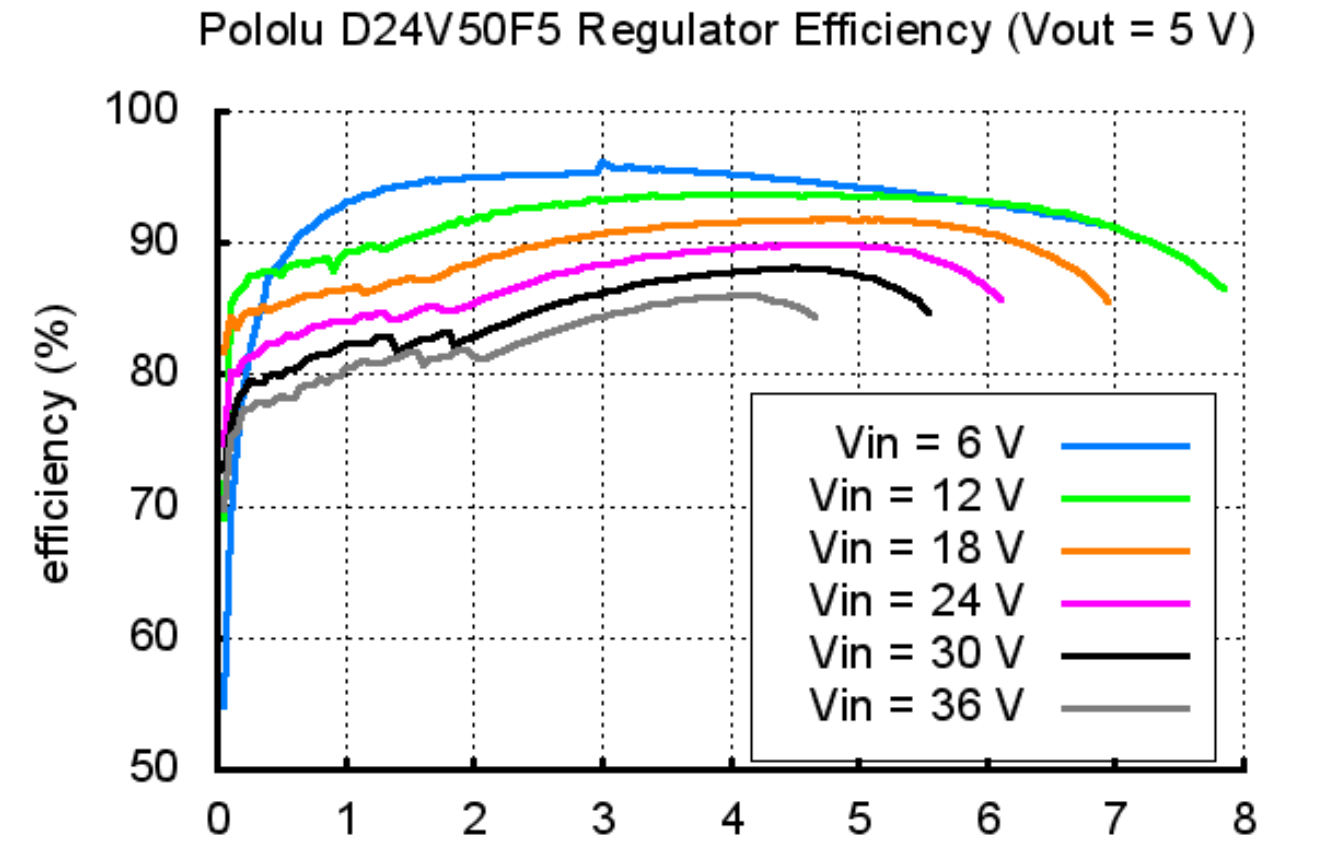
\includegraphics[width=0.5\textwidth]
	{resources/D24V50F5.PNG}
	\caption[Wirkungsgrad D24V50F5]{Wirkungsgrad D24V50F5 \protect\cite{D24V50F5}}
	\label{fig:D24V50F5}
\end{figure}

\subsection{Schleifring}

Damit Kabel durch eine endlos drehende Vorrichtung geführt werden können, benötigt es einen Schleifring. Da vermehrt nicht nur Speisung, sondern auch Datenübertragung über Schleifringe geführt werden, wächst dieses Sortiment stetig. Es gibt bereits einige Hersteller aus dem amerikanischen und asiatischen Markt, welche Gigabit-Ethernet Schleifringe vertreiben. Ein Ethernet-Schleifring, der zusätzlich Leistungsübertragung bis 5A zulässt kostet nach Abklärungen bei diversen Herstellern zwischen 120 - 500 Fr.    


\section{Zwischenfazit}
\label{ZwischenfazitInfo}
Für die Einarbeitung in das Projekt ist die Informationsbeschaffung bzw. Recherche ein wesentlicher Bestandteil. Dabei werden wichtige Grundlagen für die Konzeption erstellt. Mittels Schrittmotoren oder Gleichstrommotoren kann der Velodyne gedreht werden. Für die Datenverarbeitung stehen mehrere Einplatinencomputer zur Verfügung, dabei muss jedoch die Integration in das System gewährleistet sein. 